\documentclass{report}
\usepackage[margin=1.25in]{geometry}
\usepackage{hyperref}
\usepackage{amsmath}
\usepackage{amssymb}
\usepackage{amsthm}
\usepackage{listings}
\usepackage{parskip}
\usepackage{graphicx}
\usepackage[center]{caption}

\newcommand\imageheight{10cm}

\newtheorem{thm}{Theorem}
\title{+/ Drawings}
\author{Varik Valefor}
\begin{document}
\maketitle{}
\tableofcontents{}
\chapter{le tepavroipli}
.ni'o ti poi tetcidu cu vasru su'o lo lampru pixra poi se zbasu la .varik.\ .valefor.\ ku'o goi ko'a ge'u .e lo datni po ko'a

.i le nu zo su'o sepilno cu krinu le nu su'o da poi se zbasu la .varik.\ .valefor.\ ku'o zo'u selcaugau da ti poi tetcidu\@  .i le nu selcaugau lo glefi'a pixra poi se zbasu la .varik.\ ku'o ti poi tetcidu cu mupli
\chapter{la'o gy.\ 20200414042645-03 .gy}
\begin{figure}[ht]
	\centering
	
\includegraphics[height=\imageheight]{20200414042645-03/20200414042645-03.jpg}
	\caption[center]{le cipra pixra noi claxu lo xamgu cmene}
\end{figure}
\section{le pamoi veskicu po le pixra}
.ni'o ti poi pixra cu pu sezbasu ki'u le nu djica le nu jdice le du'u le nu pilno lo skami smacu le nu pixra cu frili kei kei .e le nu la'o gy.\ GIMP .gy xlali samru'e \@ .i le du'u la'o gy.\ GIMP .gy xlali samru'e kei .e le du'u le nu pilno lo skami smacu le nu pixra cu tcecumki cu sejimpe                                                     i

.ni'o nelci la'o gy.\ dickcissel .gy
\section{le jacba'a}
.ni'o la .varik.\ jinvi le du'u le jacyba'a po ti poi pixra cu toltce dukse\ldots\@ .i le nu di'u tceje'u cu cabna le nu la .varik.\ pensi le du'u la .varik.\ pu fatri lo favytcinymupli po ti poi pixra poi claxu le jacyba'a
\begin{figure}[ht]
	\centering
	
\includegraphics[height=10cm]{20200414042645-03/20200414042645-03-uw.png}
	\caption[center]{.ni'o lo favytcinymupli po le pixra cu segubyternoi\ldots i le kerfa bo tengu claxu cu go'i\@  .i rigni}
\end{figure}
\chapter{la'o gy.\ Proactive Security .gy}
\begin{figure}[ht]
	\centering
	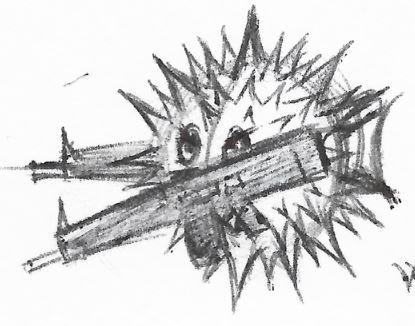
\includegraphics[height=10cm]{proactivesecurity/proactivesecurity.png}
	\caption[center]{.ni'o le nu mi'a pilno la'o gy.\ OpenBSD .gy cu zva'ati\@  .i doi fazgau do'u ko na troci}
\end{figure}
\section{le pamoi velski po le pixra}
.ni'o le jongau pixra cu sekibdu'a ki'u le nu filselga'e claxu lo pixra poi pixra la .pyfis.

.ni'o la .pyfis.\ claxu lo kalmebykre ki'u le nu mo'ifli le nu pixra lo kalmebykre

.ni'o la'o gy.\ AA-12 .gy u'enderfu xacyce'a
\chapter{la'o gy.\ WESTERNUNIONSOFTHECOUNTRYWESTERNS .gy}
\begin{figure}[ht]
	\centering
	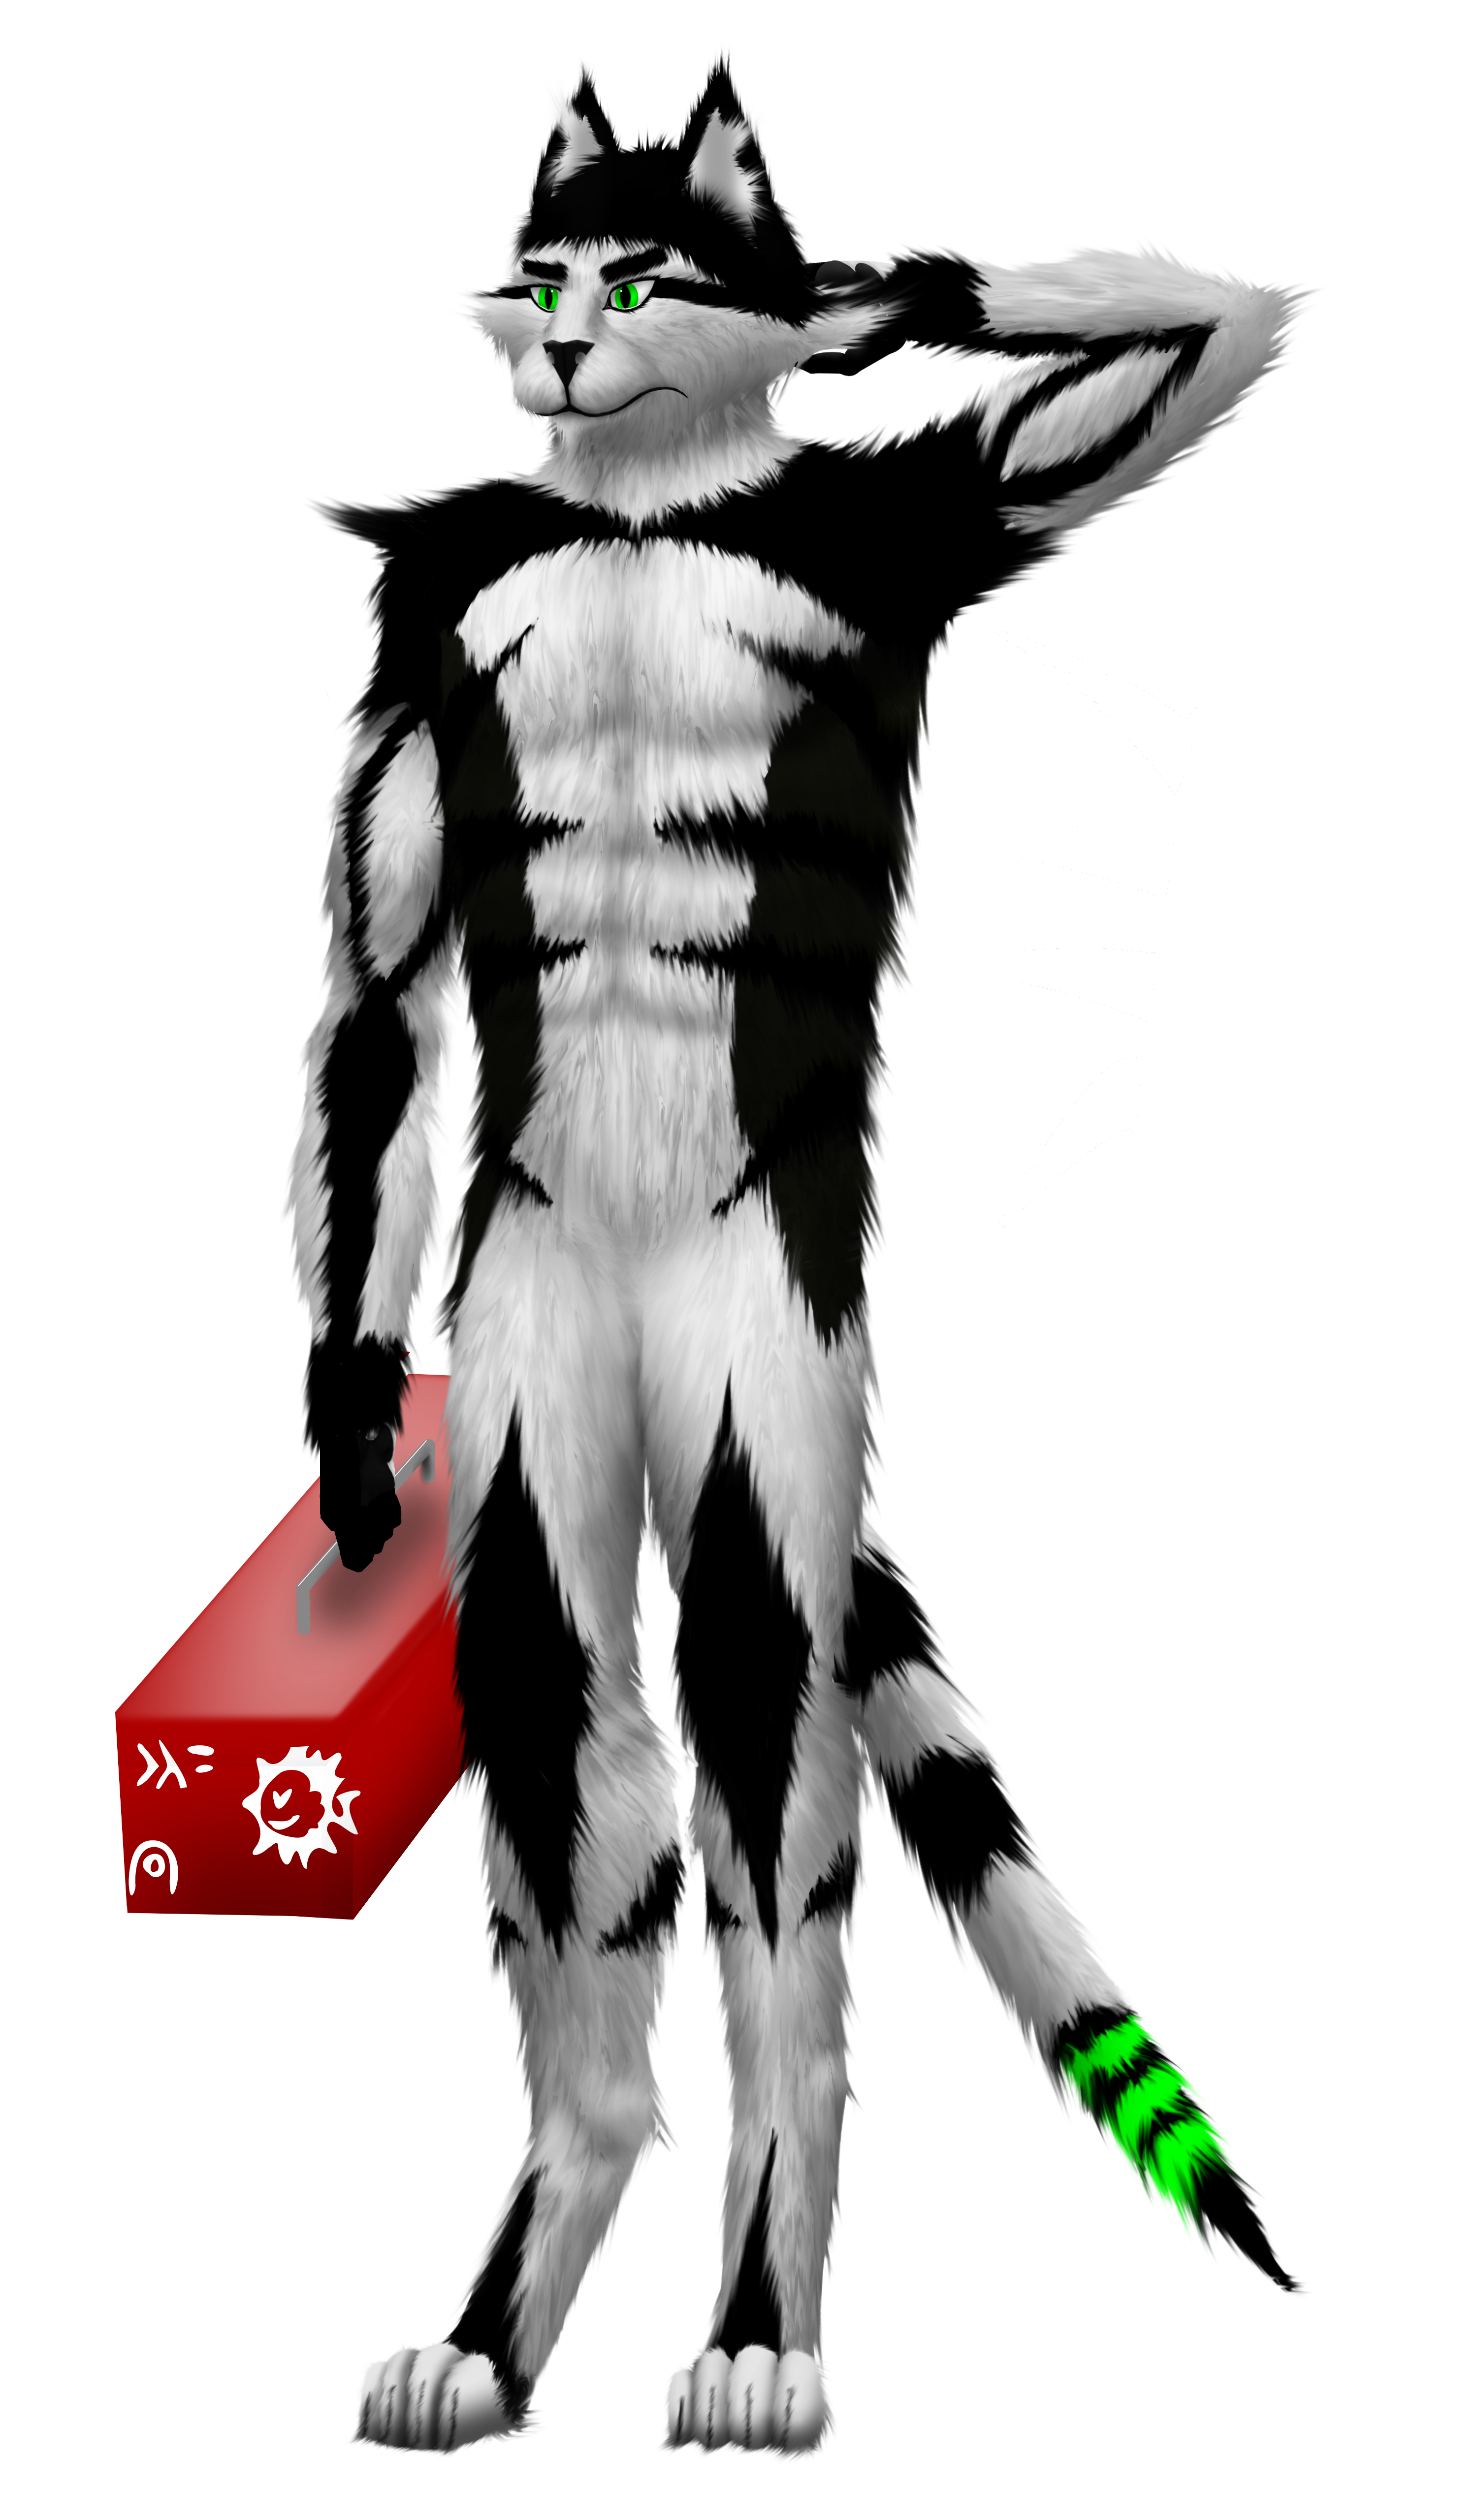
\includegraphics[height=\imageheight]{50x/toolbox/westernunionsofthecountrywesterns.png}
	\caption[center]{le pixra .e le na setcidu}
\end{figure}
\section{le pamoi velski po le pixra}
\subsection{lo snada ci fi'u vo zo'e}
.ni'o le nu la .varik.\ troci le nu pixra lo ci fi'u vo xarpre po la .varik.\ kei gi'e denpa fe le nu pixra cu semulcabna le nu la .varik.\ pixra lo ci fi'u vo xarpre po la .varik.
\subsection{le jacyba'a .e le pilno jaspu}
.ni'o ji'a ti poi pixra cu na mutce fanza se jacyba'a\@  .i ku'i ti poi pixra cu na sevasru la'o gy.\ public domain .gy\@  .i la .varik.\ ralte le krali po ti poi pixra\@  .i ku'i le nu li ni'e ni di'u jetnu lo'o selbi'o cu cumki\@  .i le nu le temci cu flecu pe'a cu cabna le nu li ni'e ni la .varik.\ nelci le nu la'o gy.\ public domain .gy vasru lo pixra lo'o zenba
\subsection{le pilno}
.ni'o pilno la'o gy.\ Krita .gy noi mutce to'e se nelci la .varik.

.ni'o le nu zbasu ti poi pixra cu cabna le nu la'o gy.\ Krita .gy goi ko'a ge'u nasru'e naspli masno\@  .i semupli le du'u le nu ko'a rinka le nu lo senta pe'a cu selvisnalka'e cu snidu li ji'i cino\@  .i le masna cu milxe serinka le nu la .varik.\ pilno la'o gy.\ GIMP .gy le nu zbasu lo balvi pixra\@  .i la .varik.\ ponse lo seplijaspu po la'o gy.\ CLIP STUDIO PAINT EX .gy gi'e zmanei la'o gy.\ CLIP STUDIO PAINT EX .gy la'o gy.\ Krita .gy lo so'e krinu\@  .i li ni'e ni la .varik.\ nelci la'o gy.\ WINE .gy po la'o gy.\ FreeBSD .gy lo'o ranji zenba

.ni'o le nu la'o gy.\ GIMP .gy ze'i pilno cu semulcabna le nu la'o gy.\ GIMP .gy claxu lo su'o jicmu poi sepilno la .varik.\@  .i le zmiku klina senta tadji cu semupli\@  .i krinu le nu la .varik.\ pilno la'o gy.\ Krita .gy le nu mulgau ti poi pixra
\subsubsection{lo zoi gy.\ open-source .gy sampla cu cumki xamgu}
.ni'o le zoi gy.\ open-source .gy sidbo cu senelci.\ gi'e cumki friti lo jetnu kalci pe'a\@\@  .i lu lo prenu poi to'e nelci ku'o cumki cikre lo samru'e li'u xlali krinu ki'u le nu su'o da poi pilno lo samru'e zo'u da na samru'e ciska\@\@  .i ji'a lo xlali samselpla cu zasti\@  .ije la .varik.\ na jinvi le du'u le samselpla po la'o gy.\ Krita .gy cizra xamgu

.ni'o le nambi cu secusku ki'u le nu la .varik.\ djica le nu la .varik.\ nelci la'o gy.\ Krita .gy .e la'o gy.\ GIMP .gy.\\@  .i ku'i la .varik.\ nelci la'o gy.\ Krita .gy .e la'o gy.\ GIMP .gy .inaja la'o gy.\ Krita .gy .e la'o gy.\ GIMP .gy sisti le nu kalci pe'a
\subsection{le sinxa}
.ni'o le nu sispe'i zo'e poi sesinxa le sinxa cu frili le tcidu
\subsection{le versiio bo jitro pilno}
.ni'o secumki le nu le citri po ti poi pixra ku sekibdu'a fi la'o gy.\ GitHub .gy\@  .i la .git.\ jitro ti poi ti pixra gi'e zbasu le mlitce barda citri bo datnyveiste
ku'i le nu le citri cu tolkli ku cumki ki'u le nu la .varik.\ djica le nu la .varik.\ frili cple'idju zo'e poi indika le du'u la .varik.\ pu zbasu ti poi pixra
\subsection{le nitpiki}
.ni'o le xamgu nitpiki cu mutce senelci\@  .i ku'i la .varik.\ djica le nu le nitpiki cu tilcfu ki'u le nu la .varik.\ jinvi le du'u li ni'e ni lu le caltai po le birka ku ku namapti le ctino po le birka li'u goi ko'a sidju cu dubmau li ni'e ni lu le birka cu xlali li'u goi ko'e sidju\@  .i ku'i ko'a .e ko'e cumki sidju
\subsection{le pilno}
.ni'o pilno la'o gy.\ ed(1) .gy le nu ciska ti poi celski
\section{le xlali betfu bo sluji}
le caltai po le betfu sluji po la'o gy.\ VUNC .gy ku po la'o gy.\ WESTERNUNIONSOFTHECOUNTRYWESTERNS .gy xlali

.i le nabmi cu serinka le tadji po le nu pixra lo betfu sluji kei po la .varik.\ ku ku goi ko'a\@  .i ko'a pruce fo le nu pixra lo nonkansa pe'a sluji
\section{le sutra pirlarfi'i}
le lisri skina poi skicu le pruce po le nu zbasu la'o gy.\ WESTERNUNIONSOFTHECOUNTRYWESTERNS .gy cu kibzva la'o gy.\ \url{https://diode.zone/w/vR9yipHTfuaH3SKPiEXFLm} .gy .e la'o gy.\ \url{https://vimeo.com/635651456} .gy\@  .i ku'i ji'a lo gletu pe'a jifkri goi ko'a cu cumki catlu le skina ki'u le nu le skina kibzva la'o gy.\ \url{https://www.youtube.com/watch?v=0wyF7okop64} .gy
\subsection{le mabla skicu}
.ni'o le skina pagbu po le sutra pirlarfi'i cu milxe mabla le demri'a

.ni'o le xlali cu lakne sekrinu le nu la .varik.\ pilno le la'o gy.\ AVI .gy pruce poi claxu lo sumti ku'o po la'o gy.\ \textsc{ffmpeg} .gy goi ko'a le nu rejgau le lisri skina\@  .i ko'a pilno le mutce cirko bo rinka bo pruce po la'o gy.\ H.264 .gy
\section{le sirsunla tcila claxu}
.ni'o le sirsunla po la'o gy.\ VUNC .gy ge'u po ti poi pixra cu nacmatilcfu

.ni'o le nu zbasu la'o gy.\ WESTERNUNIONSOFTHECOUNTRYWESTERNS .gy cu cabna le nu la .varik.\ filba le nu jmina lo cmalu sirsunla bo tcila\@  .i le filba cu serinka le pixra poi sevasru noda .e le barda sirsunla tcila
\section{le tsautu}
\subsection{le pamoi tsautu}
.ni'o le pamoi versiio po la'o gy.\ WESTERNUNIONSOFTHECOUNTRYWESTERNS .gy cu milxo mabla pinsi bo tsautu
\begin{figure}[ht]
	\centering
	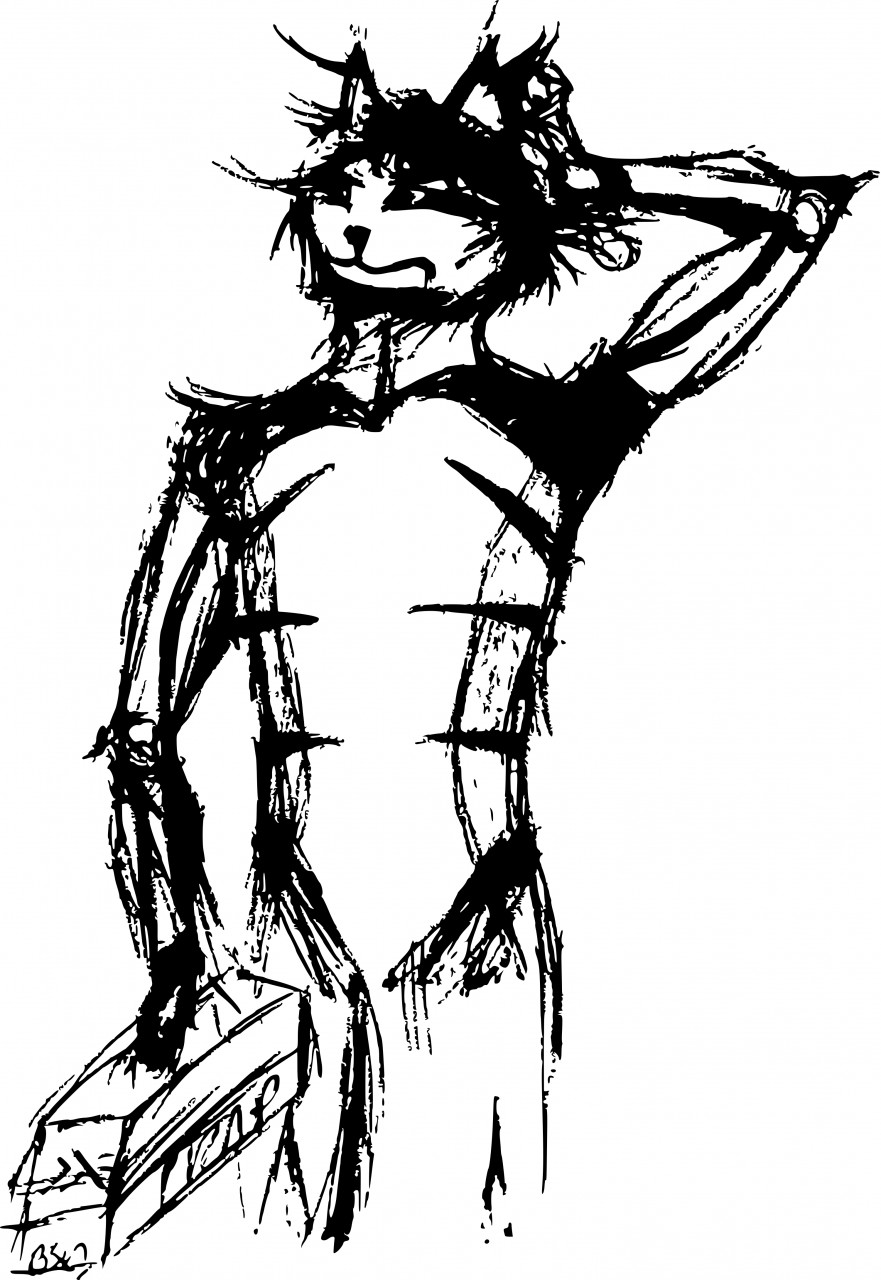
\includegraphics[height=\imageheight]{50x/toolbox/s1v1.jpg}
	\caption[center]{le pamoi versiio po la'o gy.\ WESTERNUNIONSOFTHECOUNTRYWESTERNS .gy}
\end{figure}
\subsection{le remoi tsautu}
.ni'o le pamoi tsautu po la'o gy.\ WESTERNUNIONSOFTHECOUNTRYWESTERNS .gy cu pamoi milxo xamgu pinsi bo tsautu\@  .i ku'i ti poi tsautu cu uaigri le vektori pixra poi kibzva la'o gy.\ \url{https://github.com/varikvalefor/drawingstuff/blob/master/50x/toolbox/toolboxsketch002.svg} .gy
\begin{figure}[ht]
	\centering
	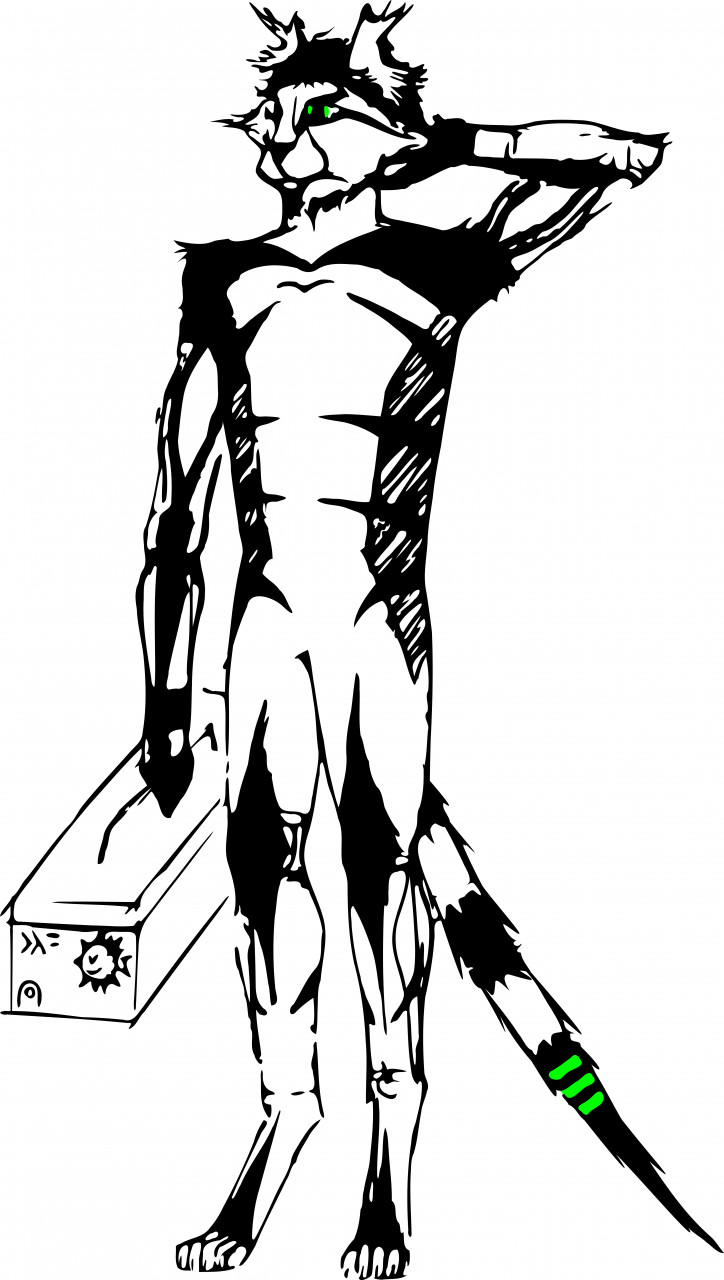
\includegraphics[height=\imageheight]{50x/toolbox/s1v2.jpg}
	\caption[center]{le pamoi tsautu po la'o gy.\ WESTERNUNIONSOFTHECOUNTRYWESTERNS .gy}
\end{figure}
\chapter{la'o gy.\ HOLLYWOODFREAKSONTHEHOLLYWOODSCENE .gy}
\begin{figure}[ht]
	\centering
	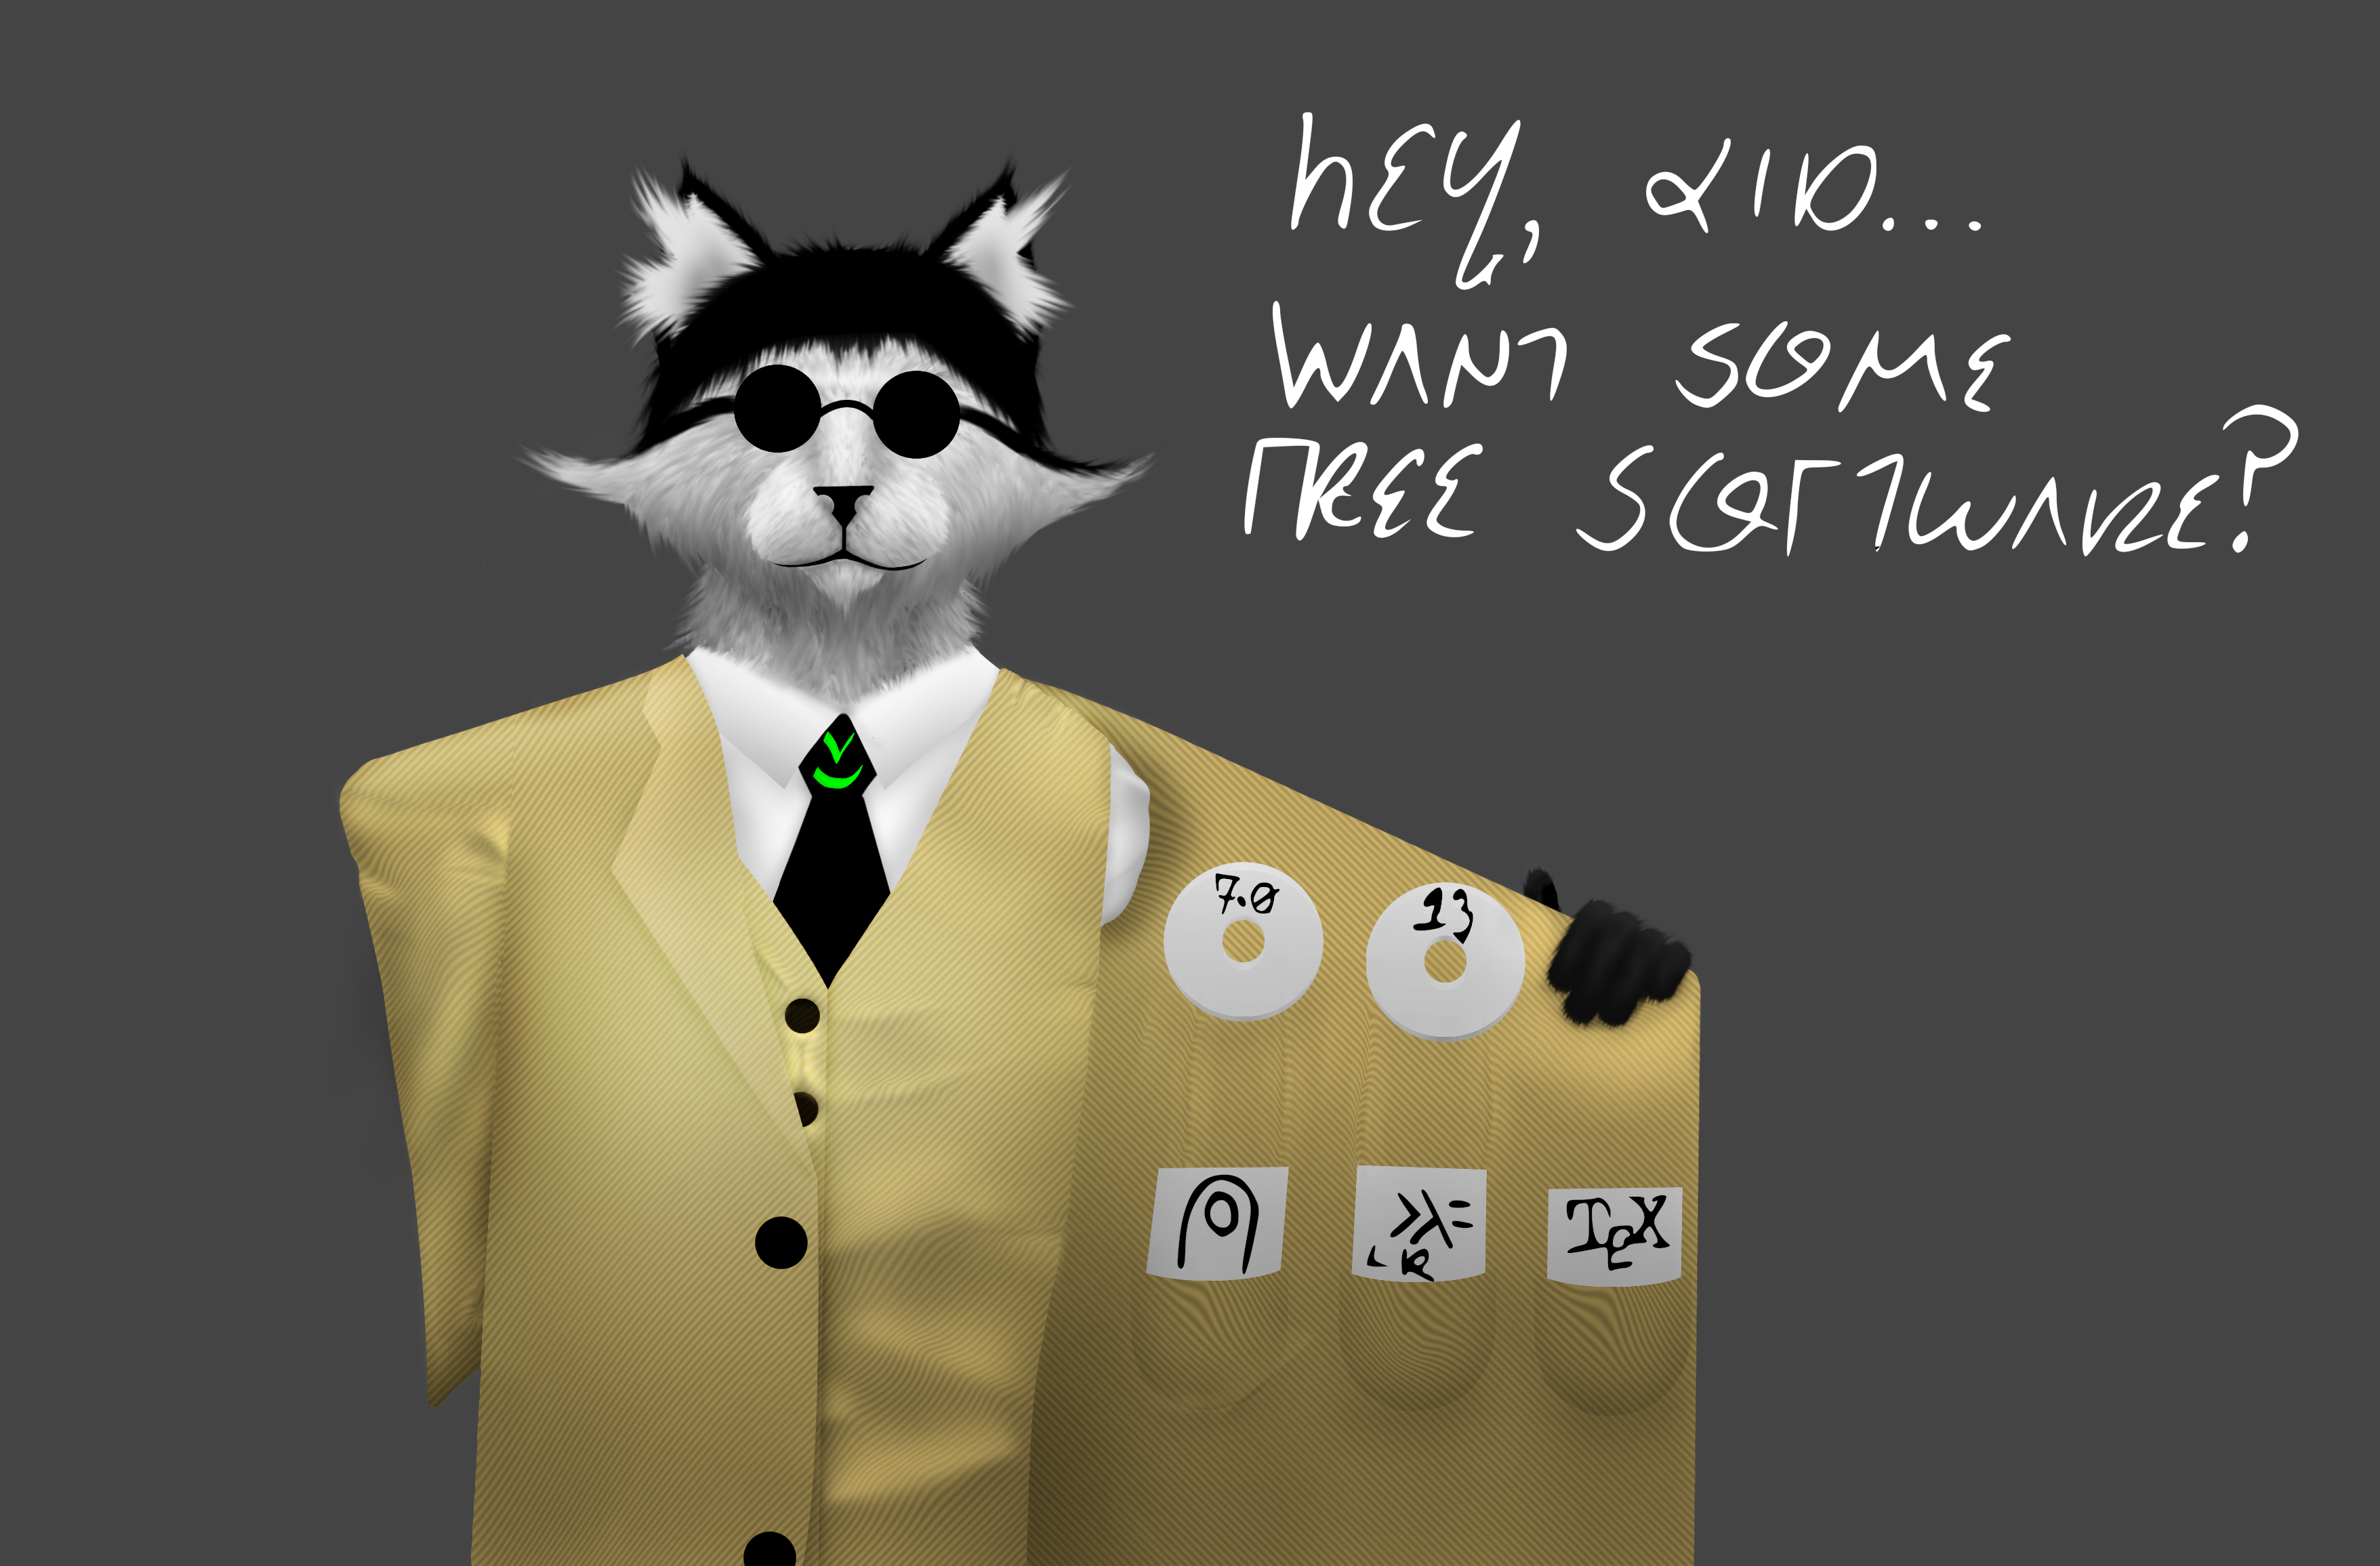
\includegraphics[height=\imageheight]{hollywoodfreaksonthehollywoodscene/hollywoodfreaksonthehollywoodscene.png}
	\caption[center]{la'o gy.\ HOLLYWOODFREAKSONTHEHOLLYWOODSCENE .gy}
\end{figure}
\section{le pamoi velski po le pixra}
\subsection{le bebna ba'e tordu lisri}
.ni'o le ctemidju cu tcika le nu lo prenu goi ko'a cadzu lo klaji\@  .ije ko'a jibni lo dikca bo fatri dinju\@  .ije le prenu poi se viska lo tcidu ku'o goi ko'e klama ko'a lo cmatricu
.i ko'a simlu le nu selspaji\@  .ije ko'e tcuskuue lu doi le verba\@  .i xu do se seldji lo fingubni proga li'u
.i le tcidu cu cumki jivbi'o le du'u fitytu'i gi'a na fitytu'i
\subsection{la'o gy.\ Blah .gy}
.ni'o lo bebna sexamsku cu segubnoi

.ni'o ti poi pixra cu bebna sexamsku gi'e pamoi ba'e jetnu bo troci bo se pixra lo bukpu la .varik.
\subsection{le daski sevasru}
.ni'o le cukmirvelvei poi se tcita zoi gy.\ 7.0 gy.\ cu cukmirvelvei la'o gy.\ OpenBSD .gy\@  .i le cukmirvelvei poi se tcita zoi gy.\ 13 .gy cukmirvelvei la'o gy.\ FreeBSD .gy
\subsubsection{le cuktermai}
.ni'o la .varik.\ djica le nu le pixra cu sitna le ziljmina proga kei ca'o le nu la .varik.\ zbasu fo'a\@  .i da poi sidbo zo'u da na temsepcau mulno pe'a
\subsubsection{le kosta daski}
.ni'o le tcidu cu sruma le du'u lo daski sevasru cu papri goi ko'a poi krati sesamrkompli po le skami bangu poi secusku
\subsubsection{li ni'e ni co'e}
.ni'o le nu la .varik.\ djica le nu le pixra cu sitna le ziljmina proga kei cabna le nu la .varik.\ zbasu fo'a\@  .i ku'i da poi sidbo zo'u da na temsepcau mulno pe'a
\subsection{lo cfilyfacki}
.ni'o lo cfilyfacki cu roroi zanvi'e
\subsection{le pilno}
.ni'o pilno la'o gy.\ GIMP .gy le nu zbasu ti poi pixra

.ni'o pilno la'o gy.\ ed(1) .gy le nu ciska dei
\section{le taxfu poi claxu le ci cimde pe'a}
.ni'o lo so'o prenu xusra le du'u le taxfu po la'o gy.\ VUNC .gy ku'o po la'o gy.\ HOLLYWOODFREAKSONTHEHOLLYWOODSCENE .gy claxu le ci cimde pe'a gi'e simlu pelji .a zo'e

.i la .varik.\ tugni fi te xefamsku

.i .o'u le nu dasni lo vejmina po lo pelji kista .e lo pelji nercreka .e lo pelji creka ge'u poi claxu lo trixe cu mutce xamji
\section{le ctino po le cukmirvelvei}
.i la .varik.\ jinvi le du'u le velvei cu tamsmi lo pelji .e narcukmirvelvei\@  .i le nabmi cumki serinka le tcenarkli po le velvei
\chapter{la'o gy.\ BROKEDOWNOUTINADITCHOFOLDRUBBISH .gy}
\begin{figure}[ht]
	\centering
	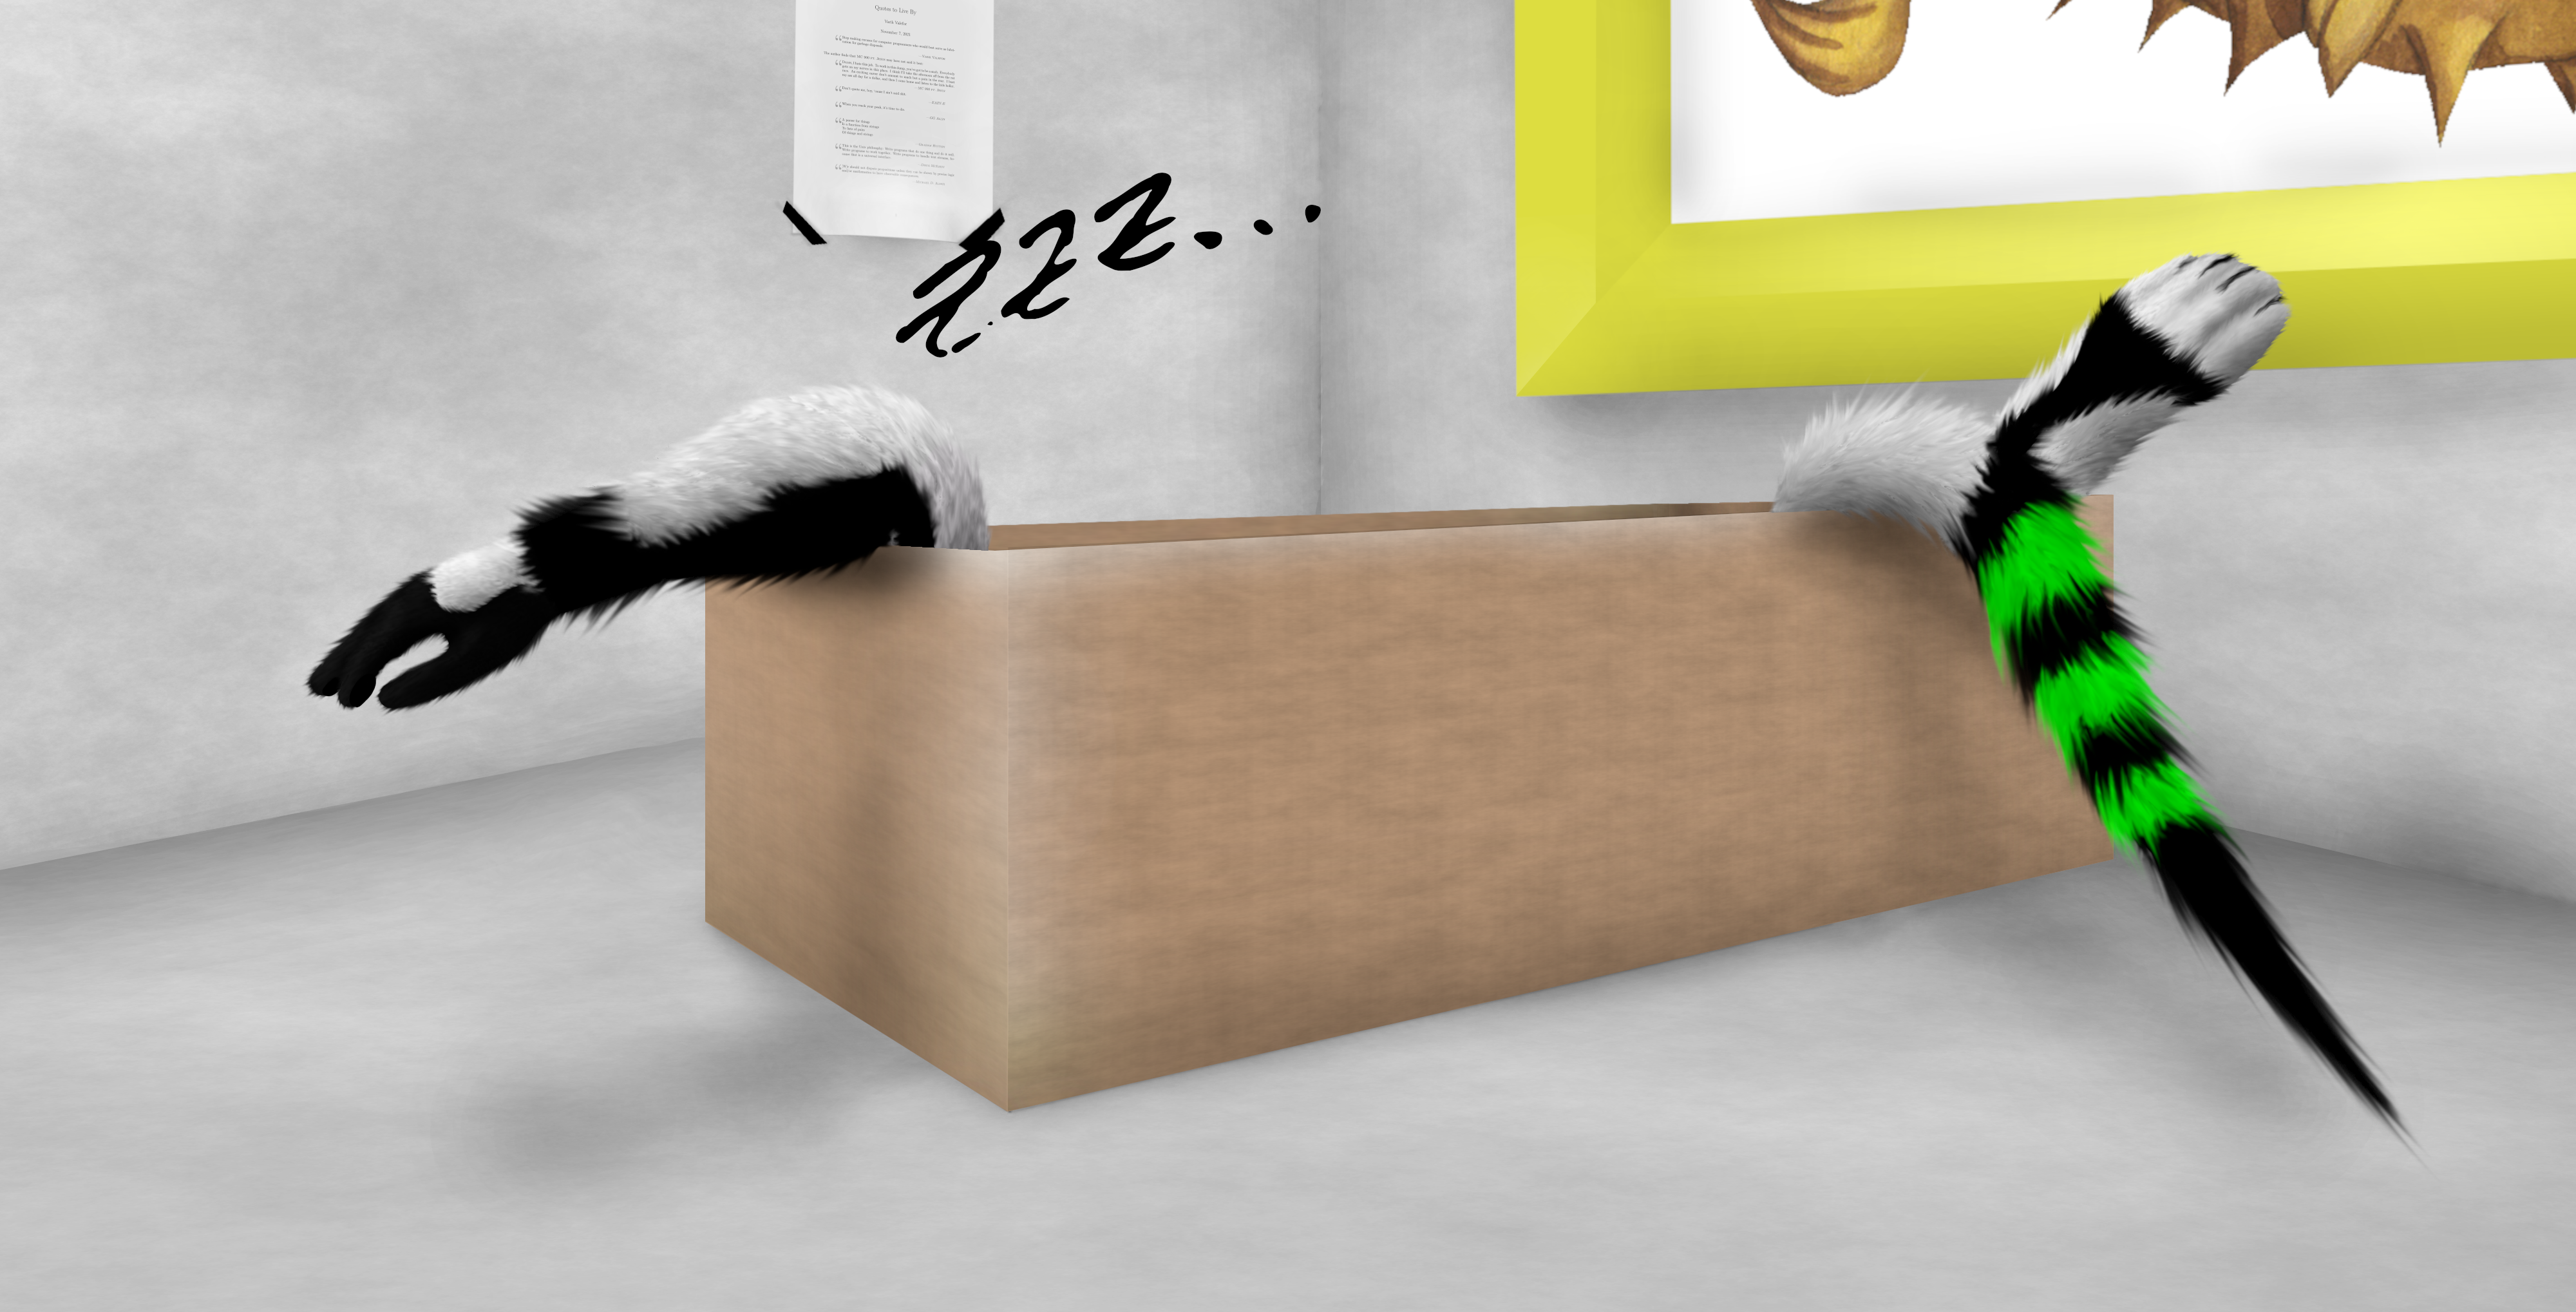
\includegraphics[width=\textwidth]{brokedownoutinaditchofoldrubbish/brokedownoutinaditchofoldrubbish.png}
	\caption[center]{.i ti poi pixra cu du le pixra\@  .i xu zo'e poi kacmyxra lo xajnuj cu sekanpe\@  .i doi bebna ko na bebna}
\end{figure}
\section{le pamoi velski po le pixra}
.ni'o lo cnino pixra cu gubni
\subsection{le jetnu pe'a trixe pixra...e lo xamsku}
.ni'o ti poi pixra gi'e secmene zoi gy.\ BROKEDOWNOUTINADITCHOFOLDRUBBISH .gy cu pamoi lo gubni pixra po la .varik.\ ku poi ckaji lo jetnu pe'a trixe pixra .enai lo stodi zilska .enai lo sucta\@  .i ji'a zoi gy.\ BROKEDOWNOUTINADITCHOFOLDRUBBISH .gy vasru lo so'u xamsku
\subsection{le tanxe}
.ni'o le tcidu cumki sruma le du'u le tinsypleta'e poi vasru le xarpre poi zutse cu tsagau gi'e na semarxa lo cmalu junta\@  .i ji'a le tcidu cu cumki sruma le du'u le vorme pe'a po le tanxe cu sevasru le tanxe gi'a sevimcu
\subsection{lo sevasru pe'a xamsku}
.ni'o le pamoi versiio po ti poi pixra cu sevasru pe'a xamsku\@  .i ciska le sevasru pe'a xamsku le tanxe\@  .i ku'i la .varik.\ pu uaigri jivbi'o le du'u le sevasru pe'a xamsku cu na mutce xajmi kei gi'e vimcu le sevasru pe'a xamsku
\subsection{zoi gy.\ ZZZ .gy}
.ni'o le nu zoi gy.\ ZZZ .gy zdani cu indika le du'u le xarpre cu sipsavgau\@  .i le nu le xarpre cu sipsavgau kei indika le du'u le xarpre sipna\@  .i ku'i zoi gy.\ ZZZ .gy kampu sipsav bo krati ki'u ma
\subsection{lo nitpiki}
.ni'o lo nitpiki cu za'o senelci
\subsection{le secuxna xarci pe'a}
.ni'o pilno la'o gy.\ GIMP .gy le nu zbasu ti poi pixra\@  .i pilno lo xance degji ualdo le jetnu pe'a pixra bo gunka

.ni'o pilno la'o gy.\ ed(1) .gy le nu ciska dei

.ni'o la'o gy.\ GIMP .gy .e la'o gy.\ ed(1) .gy bajra pe'a la'o gy.\ OpenBSD .gy
\chapter{la'o gy.\ DANCINGONTHEROOFSHOOTINGHOLESINTHEMOON .gy}
\begin{figure}[ht]
	\centering
	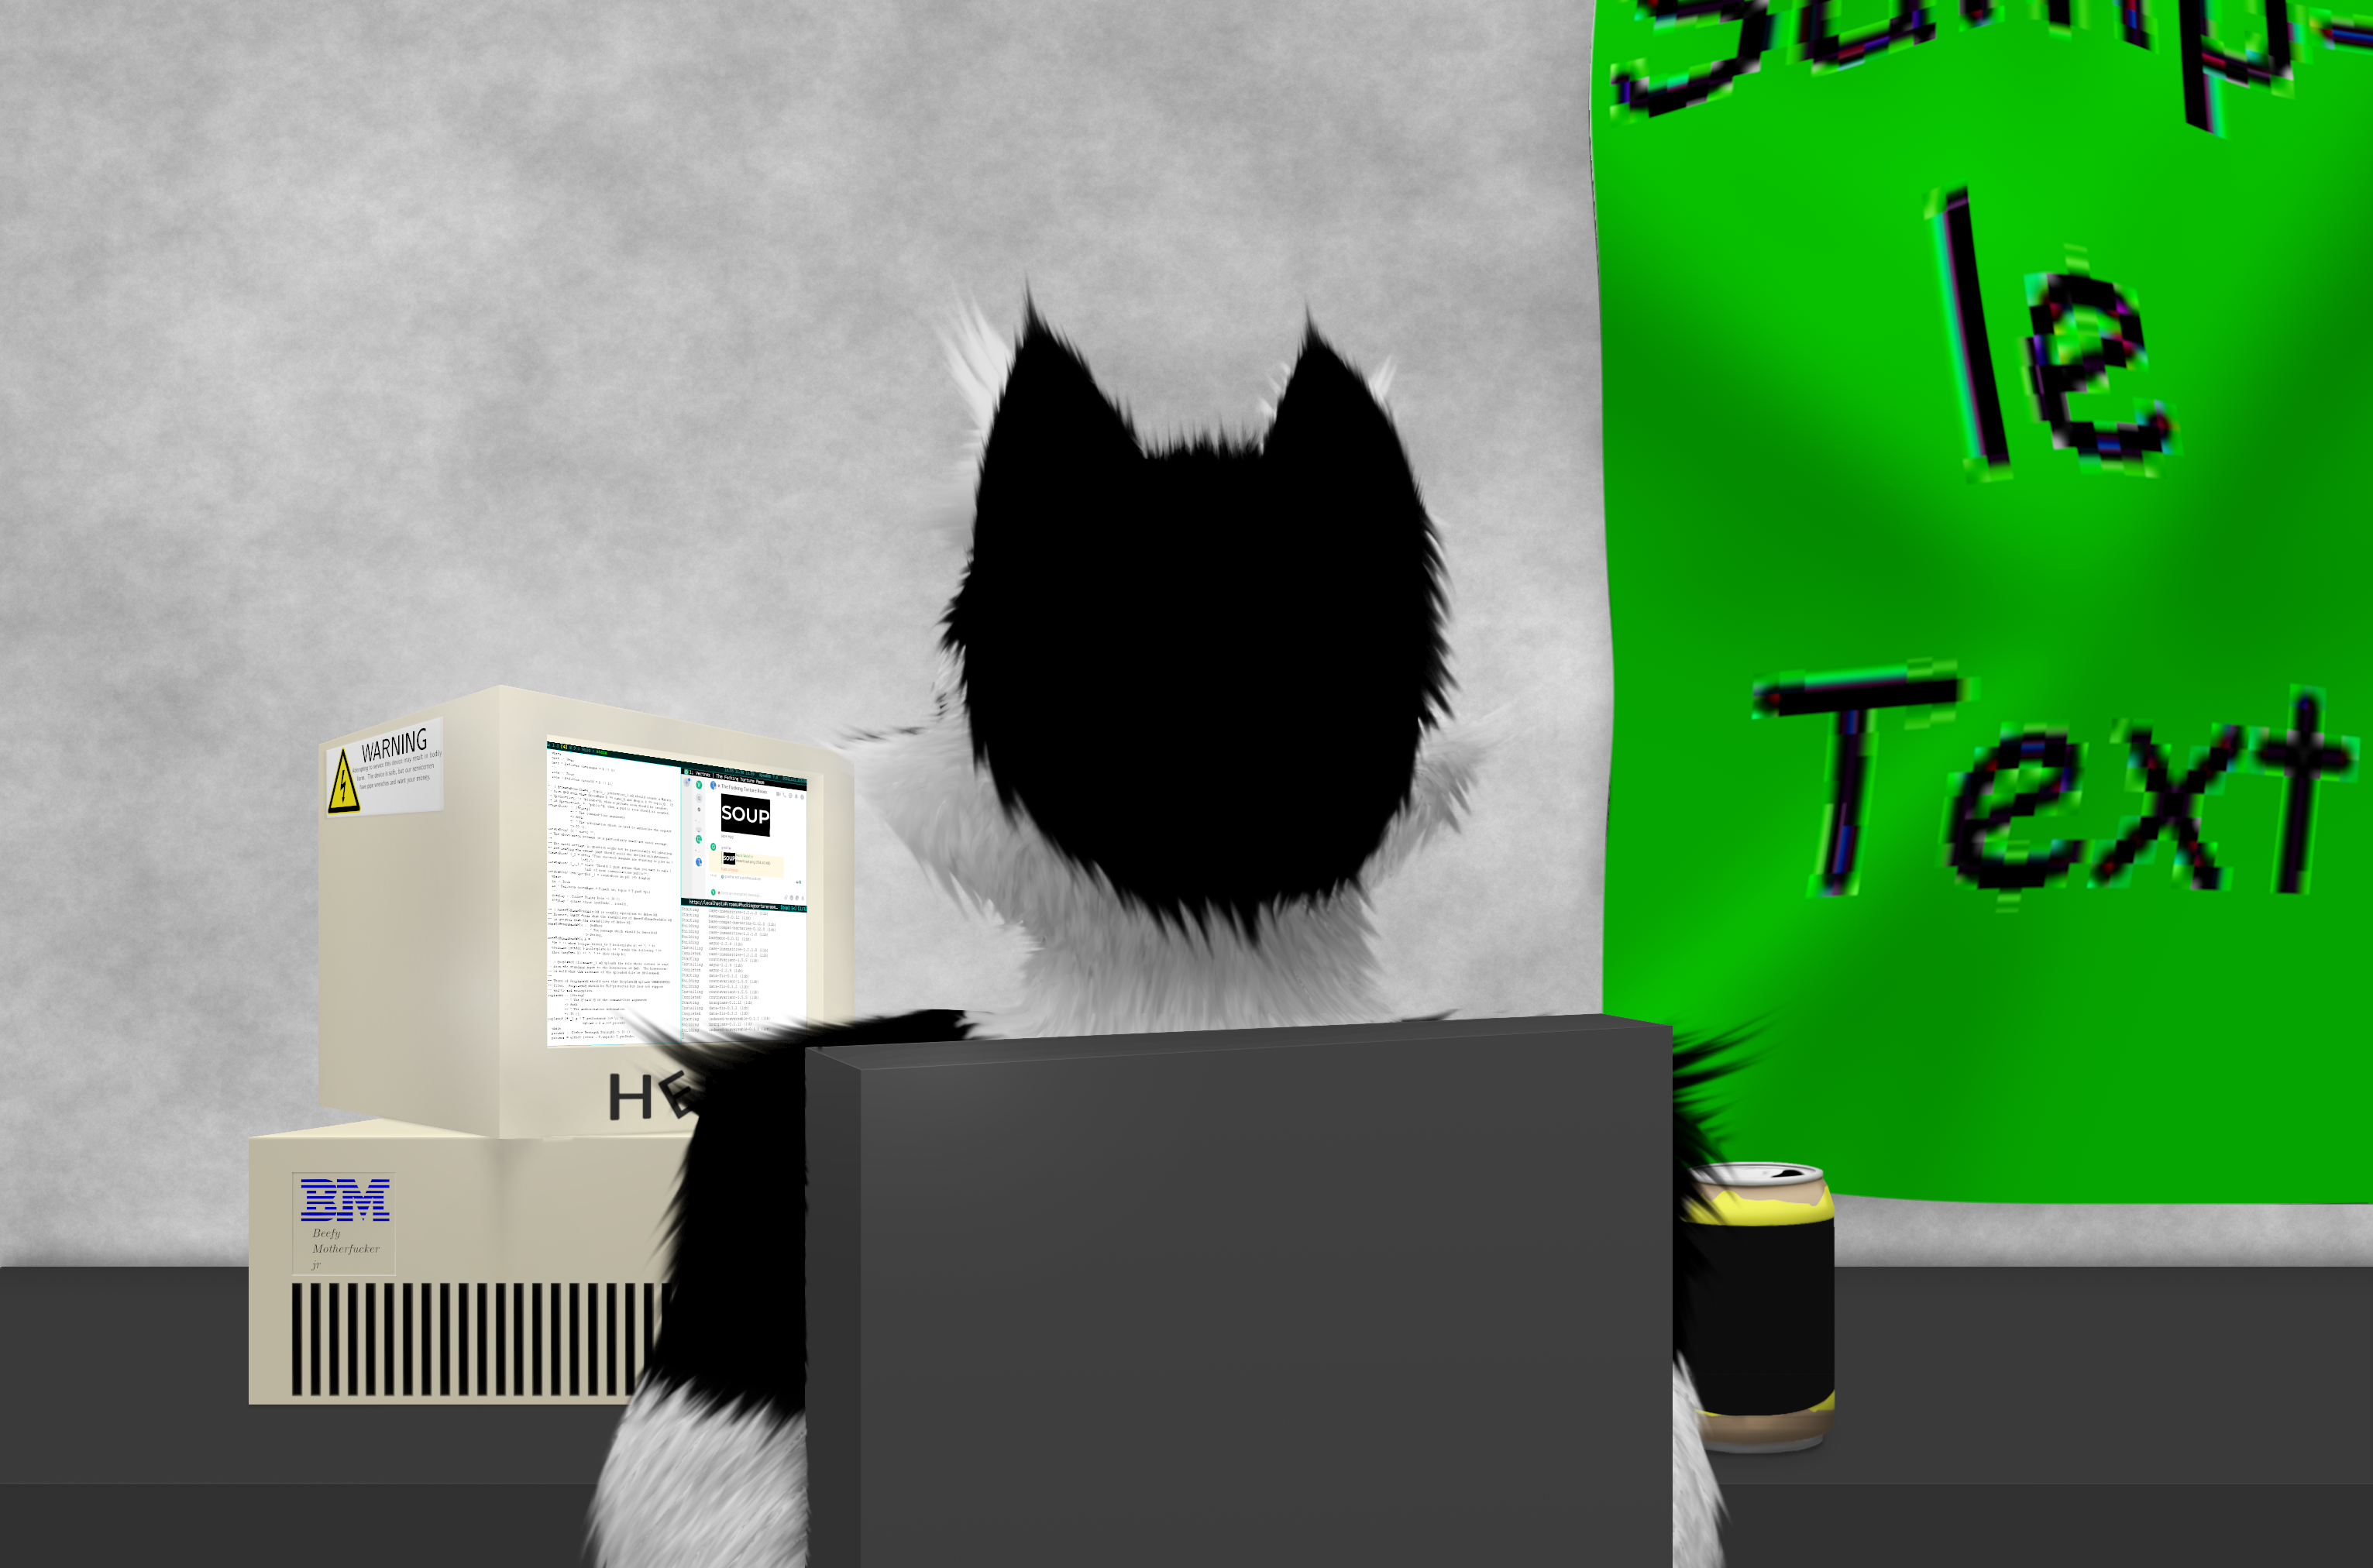
\includegraphics[width=\textwidth]{dancingontheroofshootingholesinthemoon/dancingontheroofshootingholesinthemoon.png}
	\caption[center]{.ni'o le mulbi'o versiio po la'o gy.\ DANCINGONTHEROOFSHOOTINGHOLESONTHEMOON .gy\@  .ni'o le nu viska lo ro tcila cu frili zo'e le nu pilno lo banro blaci...a lo cmactatci}
\end{figure}
\section{le pamoi velski po le pixra}
.ni'o ue'i lo ziljmina pixra cu gubni

.ni'o le pixra cu pixra lo roldje tcini\@  .i ku'i sorpa'a le nu le pixra cu na mutce tolzdi
\subsection{le vlavelcki}
zoi gy.\ VUNC .gy krati le xarpre po la .varik.
\subsection{le torveki}
.ni'o ti poi pixra cu pixra le nu la'o gy.\ VUNC .gy jibni gi'e galfi lo proga\ldots gi'e tcidu lo xlali kibzva bo notci kei
\subsection{le sexamsku .e zo'e}
.ni'o le pixra cu simsa le da'a pixra po la .varik.\ li ni'e ni sevasru sexamsku\@  .i le tcidu cumki ciksi le xamsku\@  .i ku'i ji'a ti poi pixra cu vasru le cmalu jikske bo ckipinka\@  .i ji'a le tcidu cu cumki skicu le cmalu jikske bo ckipinka
\subsection{zoi gy.\ SOUP .gy}
.ni'o zoi gy.\ SOUP .gy poi simlu lo bebna cu zvati ki'u le nu la .varik.\ na djuno le du'u sefladra le nu le pixra cu zifre vasru le pamoi kacmyxra\@  .i le nu na tenunflapai la .varik.\ cu frili la .varik.\ le nu le velski pe'a po le kacmyxra cu basti le pamoi kacmyxra

.ni'o zo velski cu sidysmu ki'u le velski pe'a cu na mutce skicu\@  .i lo zenba velski velski po le pamoi kacmyxra cu du lo'u lo tcesedemri'a kacmyxra po lo kabri poi sevasru lo alfabeta stasu le'u
\subsection{le kadje tcita}
.ni'o le setcidu po le kadje tcita cu du zoi gy.
\begin{quote}
	WARNING

	Attempting to service this device may result in bodily harm.  The device is safe, but our servicemen have pipe wrenches and want your money.
\end{quote}
.gy
\subsection{le batkyfoi}
.ni'o le pixra cu pixra le nu la'o gy.\ VUNC .gy pilno le batkyfoi\@  .i ku'i le batkyfoi naseviska\@  .i ku'i je secumki le nu le du'u la'o gy.\ VUNC .gy pilno le batkyfoi kei zenba xamgu seindika
\subsection{le nitpiki}
.ni'o lo nitpiki cu za'o senelci
\subsection{le seplijaspu}
.ni'o ti poi pixra cu sexrapra gi'e seplijaspu la'o gy.\ CC BY-NC 4.0 .gy\@ .i le mulno tcidu po ti poi seplijaspu cu xabju pe'a la'o gy.\ https://creativecommons.org/licenses/by-nc/4.0/legalcode .gy
\subsection{le pilno}
.ni'o pilno la'o gy.\ GIMP .gy le nu zbasu ti poi pixra\@  .i la'o gy.\ GIMP .gy tcexla\@  .i ku'i za'a la'o gy.\ GIMP .gy traji le ka ce'u xamgu pixra bo fingubni bo proga

.ni'o pilno la'o gy.\ ed(1) .gy le nu zbasu dei

.ni'o la'o gy.\ GIMP .gy .e la'o gy.\ ed(1) .gy bajra pe'a la'o gy.\ OpenBSD .gy
\section{le stizu}
.ni'o le nu le stizu poi sezutse la'o gy.\ VUNC .gy cu claxu lo tcila cu serinka le nu le stizu tengu cu ambigu'o\@  .i le stizu se.enge cu sestaile\@  .i la .varik.\ mutce nelci lo dijyzbaske po la'o gy.\ Brutalism .gy\@  .i ku'i krici le du'u le stizu cu mabla
\chapter{la'o gy.\ ITHINKWEREGOINGCRAZY .gy}
\begin{figure}[ht]
	\centering
	\includegraphics[height=10cm]{ithinkweregoingcrazy/ithinkweregoingcrazy.png}
	\caption[center]{la'o gy.\ ITHINKWEREGOINGCRAZY .gy}
\end{figure}
\section{The Original Description of the Drawing}
.ni'o zoi gy.\ BLOCKED BY SHODAN LEVEL SECURITY .gy
\subsection{lu mi viska ma li'u}
.ni'o ti poi pixra cu pixra le nu le xarpre po la .varik.\ smimlu la'o gy.\ SHODAN .gy po la'o gy.\ \textit{System Shock} .gy le ka jorne lo jimsko kei .e le ka senunfirsku fi lo nutli
\subsection{le tcika}
.ni'o ji'i za'a le pavrelmasti cu vasru pe'a lo su'o pa pixra
\subsection{le citri}
\subsubsection{le tsautu}
.ni'o lo pamuki'oki'o nanca cu sepuvza le nu la .varik.\ gubni le tsautu poi pixra le nu la'o gy.\ VUNC .gy simlu la'o gy.\ SHODAN .gy po la'o gy.\ \textit{System Shock} .gy le ke jorne lo jimsko
\subsubsection{le pamoi setroci segalfi}
.ni'o la .varik.\ tolsti le nu galfi le tsautu lo jetnu pe'a pixra\@  .i ku'i le nu la .varik.\ zbasu lo nurfu'i cu sepurci snuti vimcu le datni po le cukmakyvelvei po le ralju skami po la .varik.\@  .i ja'e le pamoi versiio po le pixra cu lakne cimni bo farcri pe'a
\subsubsection{le remoi setroci segalfi}
.ni'o li papa pi'e vo pi'e renorepa cu detri le nu la .varik.\ tolsti le nu galfi le tsautu lo jetnu pe'a pixra gi'e jmina lo tsautu poi nasevasru lo sirsunla lo samrxra po la'o gy.\ Scalable Vector Graphics .gy\@  .i snada le nu mulno le pruce
\subsubsection{le nu troci le nu jmina lo tcila}
.ni'o li ji'i re pi'e xa pi'e renorepa cu detri le nu la .varik.\ galfi le samrxra po la'o gy.\ Scalable Vector Graphics .gy lo samrxra po la'o gy.\ XCF .gy gi'e tolsti le nu jmina lo tcila\@  .i le nu jmina lo tcila cu lidne le nu jmina lo jimsko kei ki'u zo'e

.ni'o lo jetnu pe'a nabmi ku sotmei\@  .i ku'i la .varik.\ nanelci le jalge po le nu jmina le tcila kei gi'e zasysti le nu zbasu le pixra
\subsubsection{le nu sesnada jmina bo tcila}
.ni'o li reze pi'e papa pi'e renorepa cu detki le nu la .varik.\ to'ezasysti le nu zbasu le pixra gi'e ku'i ninke'u jivbi'o le du'u la'o gy.\ GIMP .gy cumki kalci\ldots pe'a
\subsubsection{le nu mulgau le pixra}
.ni'o li pa pi'e pare pi'e renorepa cu detni le nu la .varik.\ xusra le du'u le pixra cu semulgau
\subsection{le nu le ti poi pixra cu tegumgau}
.ni'o ko'a goi la'o gy.\ SHODAN .gy po la'o gy.\ \textit{System Shock} .gy velfi'i le pagbu po le pixra ku poi sefinti fo ko'a\@  .i ku'i le nu la .varik.\ napilno lo pa versiio po ko'a cu cabna le nu la .varik.\ zbasu ti poi pixra\@  .i lo menli gumgau po ko'a po la'o gy.\ \textit{System Shock} .gy .e ko'a po la'o gy.\ \textit{System Shock 2} .gy cu velfi'i ti poi pixra ku'o fo la .varik.
\subsection{lo nitpiki}
.ni'o lo nitpiki cu za'o senelci
\subsection{le seplijaspu}
.ni'o ti poi pixra cu sexrapra gi'e seplijaspu la'o gy.\ CC BY-NC 4.0 .gy\@ .i le mulno tcidu po ti poi seplijaspu cu xabju pe'a la'o gy.\ https://creativecommons.org/licenses/by-nc/4.0/legalcode .gy
\subsection{le pilno}
.ni'o pilno la'o gy.\ GIMP .gy le nu majgau ti poi pixra\@ .i  la'o gy.\ GIMP .gy xlatce\@ .i ku'i zmanei la'o gy.\ GIMP .gy la'o gy.\ Krita .gy

.ni'o i ciska dei fo la'o gy.\ ed(1) .gy

.ni'o la'o gy.\ GIMP .gy .e la'o gy.\ ed(1) .gy bajra pe'a la'o gy.\ OpenBSD .gy
\section{le kanla secortu}
.ni'o so'u da poi prenu zo'u da xusra le du'u le nu da catlu la'o gy.\ ITHINKWEREGOINGCRAZY .gy kei cu sejalge le nu da cortu kei kei goi ko'a\@  .i la .varik.\ jijyji'i le du'u lo prenu poi xusra ko'a cu du'eski ko'a gi'a bilma lo kanla secortu kei ki'u le nu la .varik.\ na zatfa'i lo satci krasi po le kanla secortu
\section{le sefrati}
.ni'o le nu la'o gy.\ ITHINKWEREGOINGCRAZY .gy nasopnelsei\ldots cu cumki sekrinu le nu zo'e poi velfi'i la'o gy.\ ITHINKWEREGOINGCRAZY .gy rirci
\subsection{le velski po le sefrati}
.ni'o su'o da poi pixra fi la .varik.\ zo'u li ni'e ni lo prenu cu nelci la'o gy.\ ITHINKWEREGOINGCRAZY .gy cu dubme'a li ni'e ni lo prenu cu nelci da
\subsection{le cumki rinka po le narselnei}
.ni'o la .varik.\ jinvi le du'u le narselnei po la'o gy.\ ITHINKWEREGOINGCRAZY .gy  cu cumki sekrinu le nu zo'e poi velfi'i la'o gy.\ ITHINKWEREGOINGCRAZY .gy rirci
\begin{thm}
.ni'o selakne le du'u lo so'u prenu cu nelci la'o gy.\ ITHINKWEREGOINGCRAZY .gy
\end{thm}
\begin{proof}
${}$
.ni'o ro da zo'u ro de poi pixra zo'u ro di poi prenu zo'u le du'u de velsitsku da cu nibyti'i le du'u di mulsmujmi de nagi'a seslabu de

.ni'o ro da poi pixra zo'u le du'u lo so'u prenu ku mulsmujmi da cu nibyti'i le du'u selakne le du'u lo so'u prenu ku nelci da\footnote{.ni'o le tcidu cu sedarsygau milxe bo senpi ti poi pixra}

.ni'o so'u prenu cu slabu la'o gy.\ \textit{System Shock} .gy\footnote{.ni'o zo so'u cumki dukse bo ruble}

.ni'o la'o gy.\ ITHINKWEREGOINGCRAZY .gy velsitsku la'o gy.\ \textit{System Shock} .gy

.ni'o ja'e selakne le du'u lo so'u prenu cu nelci la'o gy.\ ITHINKWEREGOINGCRAZY .gy
\end{proof}
\chapter{la'o gy.\ JUDASTRAINWRECK .gy}
\begin{figure}[ht]
	\centering
	
\includegraphics[height=10cm]{judastrainwreck/judastrainwreck.png}
	\caption[center]{la'o gy.\ JUDASTRAINWRECK .gy}
\end{figure}
\section{le pamoi velski po ti poi pixra}
la .varik.\ jinvi le du'u le firxa'e cu melbi
\subsection{le torveki}
.ni'o su'o da poi papri bo pixra tsautu zo'u da binxo le vektori pixra poi binxo ti poi pixra

.ni'o le tcidu tanxe pe'a vasru lo toltce bo galfi notci poi pu seterbe'i la .varik.

.ni'o ti poi pixra cu sexrapra gi'e seplijaspu la'o gy.\ CC BY-NC 4.0 .gy

.ni'o doi la'o gy.\ lamer .gy ko pilno la'o gy.\ OpenBSD .gy
\subsection{le pruce poi gasnu le nu le tsautu ku binxo le mulno pixra}
.ni'o la .varik.\ majgau le pamoi tsautu ki'u le nu la .varik.\ djica le nu la .varik.\ terxra lo nasteci

.i la .varik.\ gasnu le nu le pamoi tsautu cu binxo le vektori pixra ki'u le nu la .varik.\ djica le nu la .varik.\ terxra zo'e poi trina

.i le nu la .varik.\ terxra le cabna pixra cu milxe sekrinu le nu la .varik.\ djica le nu la .varik.\ ckasu lo prenu poi cusku lo bebna preti.\ gi'a bebna pensi
\subsection{le tcidu tanxe pe'a}
.ni'o le tcidu tanxe pe'a vasru lo toltce bo galfi notci poi pu seterbe'i la .varik.

.i le nu la .varik.\ fuktra le cmoni po la'o gy.\ SIDESHOW BOB .gy cu sebalvi le nu la .varik.\ jdice le du'u le nu la .varik.\ ckasu le prenu gi'e curmi le nu le prenu ku cmecau cu filri'a le nu cmila
\subsection{le seplijaspu}
.ni'o ti poi pixra cu sexrapra gi'e seplijaspu la'o gy.\ CC BY-NC 4.0 .gy\@ .i le mulno tcidu po ti poi seplijaspu cu xabju pe'a la'o gy.\ https://creativecommons.org/licenses/by-nc/4.0/legalcode .gy
\subsection{le pilno}
.ni'o pilno la'o gy.\ GIMP .gy le nu majgau ti poi pixra\@ .i  la'o gy.\ GIMP .gy xlatce\@ .i ku'i zmanei la'o gy.\ GIMP .gy la'o gy.\ Krita .gy

.ni'o ciska dei fo la'o gy.\ ed(1) .gy

.ni'o la'o gy.\ GIMP .gy .e la'o gy.\ ed(1) .gy bajra pe'a la'o gy.\ OpenBSD .gy
\section{le selji'i be fi la'o gy.\ JUDASTRAINWRECK .gy}
.ni'o so'u lo prenu cu gubni nitpiki la'o gy.\ JUDASTRAINWRECK .gy\ldots gi'e gubni zausku la'o gy.\ JUDASTRAINWRECK .gy
\subsection{su'o lo selji'i be fi la'o gy.\ JUDASTRAINWRECK .gy}
.ni'o su'o le selji'i be fi la'o gy.\ JUDASTRAINWRECK .gy goi ko'a cu cnita dei
\begin{itemize}
	\item .i ko'a indika le du'u le selxra be fe ko'a ku goi ko'e cu mapra keitci kei ku ri'a le nu ko'a indika le du'u le kerfa be fe ko'e cu dukse 
	\begin{itemize}
		\item .i ku'i la .varik.\ toltu'i zo'e le du'u go'i
	\end{itemize}
	\item .i ko'a pixra le ambigu
	\begin{itemize}
		\item .i la .varik.\ mlitu'i zo'e le du'u go'i
	\end{itemize}
	\item .i ko'a citmle
	\begin{itemize}
		\item .i la .varik.\ no'e tugni zo'e le du'u go'i
	\end{itemize}
\end{itemize}
\section{le ctino}
.ni'o la .varik.\ jinvi le du'u cumki fa le nu li ni'e ni la'o gy.\ JUDASTRAINWRECK .gy goi ko'a vasru le ctino cu dukse kei kei .e le du'u ko'a dukse manku
\section{le xance}
.ni'o la'o gy.\ JUDASTRAINWRECK .gy indika le du'u le xance degji be fi la'o gy.\ VUNC .gy ku goi ko'a tordu  .i ku'i ko'a na tordu
\end{document}
